% !TEX root = TD_fluides_part1.tex

\setcounter{section}{4}

\section{Ecoulements visqueux II : problèmes instationnaires}

\setcounter{subsection}{-1}

\subsection{Premier problème de Stokes} 

{\em (exercice préparatoire, correction sur moodle)} 



%\subsection{Second problème de Stokes}

%--------------------------------------------------------------------------------------------------
\subsection{Ecoulement au voisinage d'une paroi oscillante (second problème de Stokes)} \label{2pbStokes}
%--------------------------------------------------------------------------------------------------

On consid\`ere un fluide de viscosit\'e cin\'ematique $\nu$ occupant un demi-espace 
limit\'e par une plaque plane anim\'ee d'un mouvement oscillant sinuso\"{\i}dal $U \cos \omega t$, 
parall\`element \`a elle-m\^eme ("deuxi\`eme probl\`eme de Stokes"). 
%Montrer que le mouvement p\'en\^etre dans le fluide sur une distance $\delta = \sqrt{2\nu/\omega}$.
Retrouvez la loi $u(y,t)$ décrivant la structure de l'écoulement (cf. tableau "solutions exactes" en Annexe).

Déduisez-en la contrainte visqueuse exercée par le fluide sur la paroi, et montrez que celle-ci est donnée par la loi suivante :

\[
\color{black}{\tau_p  = - \frac{\mu U \sqrt{2}}{\delta} \cos (\omega t - \pi/4)}
\]

Que vaut la vorticité dans l'écoulement ? montrez que la vorticité à la paroi est directement reliée à la contrainte pariétale.




%--------------------------------------------------------------------------------------------------
\subsection{Rythmes cardiaques (TP numérique)}
%--------------------------------------------------------------------------------------------------

Outre une diff\'erence de pression moyenne,
le c{\oe}ur qui bat impose une variation p\'eriodique du gradient de
pression ce qui conduit \`a un \'ecoulement puls\'e dans les vaisseaux
sanguins.
L'objectif de cet exercice est de caract\'eriser ce type d'\'ecoulement
en particulier dans les limites des basses fr\'equences (organisme au repos) 
et hautes fr\'equences (activit\'e cardiaque intense).
 
Consid\'erons un \'ecoulement plan entre deux plaques planes distantes de $2h$
g\'en\'er\'e par un gradient de pression sinuso\"{\i}dal
\`a pulsation $\omega$ fix\'ee~:
\[
\dpa{p}{x} = K \cos\omega t.
\]

\begin{enumerate}
\item 
Dans l'hypoth\`ese d'un \'ecoulement plan parall\`ele, montrer que
la vitesse horizontale $u(y, t)$ v\'erifie l'\'equation
\begin{equation}
\underbrace{\rho \dpa{u}{t}}_{[I]} = \underbrace{- K \cos \omega t}_{[P]} + \underbrace{\mu \ddpa{u}{y}}_{[V]}
\label{eq:ns}
\end{equation}

\item Comparer l'ordre de grandeur des termes $[I]$ et $[V]$ dans l'équation précédente. Montrez que le rapport de ces deux termes fait apparaître 
le nombre de Stokes (ou nombre de Womersley) $St = \frac{\omega h^2  }{\nu}$.

\item Dans l'hypothèse $St \ll 1$, justifiez que l'écoulement correspond à chaque instant à l'écoulement de Poiseuille plan   
(régime quasi-statique).

\item Dans l'hypothèse $St \gg 1$, l'analyse des ordres de grandeur suggère qu'on peut dans une première approximation
négliger le terme visqueux. Quelle est alors la solution du problème ? celle-ci est-elle valide dans la totalité du domaine ?

\item Toujours dans le cas  $St \gg 1$, justifiez qu'il existe une {\em couche limite} dans laquelle le terme visqueux ne peut être négligé. 
Quelle est l'épaisseur de cette couche limite ?

\item $^*$ Dans le cas général ($St = {\mathcal O}(1)$, montrez que la solution du problème peut se mettre sous la forme suivante :
$$u(y, t) = Re \left \{  \underline{U}(y) \e^{\im \omega t} \right \}.$$

Avec 

\begin{equation}
\label{sol}
 \underline{U}(y) = \frac{iK}{\rho \omega} \left \{ 
1 - \frac{\cosh [ y ( 1+i) \sqrt{\omega / 2\nu} ]}{\cosh [ 
h ( 1+i) \sqrt{\omega / 2\nu} ]}
\right \}
\end{equation}

Indication : on utilisera la méthode de la variable complexe comme dans le cas de l'exercice précédent pour aboutir à une équation différentielle d'ordre 2 pour $ \underline{U}(y)$ que l'on résoudra en tenant compte des conditions aux limites du problème.

\item $^*$ Etudiez le comportement de l'expression précédente dans les limites  $\omega \rightarrow 0 $ et $\omega •\rightarrow \infty$, et montrez que l'on retrouve bien les prédictions obtenues précédemment dans les cas $St \ll 1$ et $St \gg 1$.




%\begin{figure}[htb]
%  \begin{center}
 %   \begin{picture}(100, 30)(0, 50)
  %    \put(0, 0){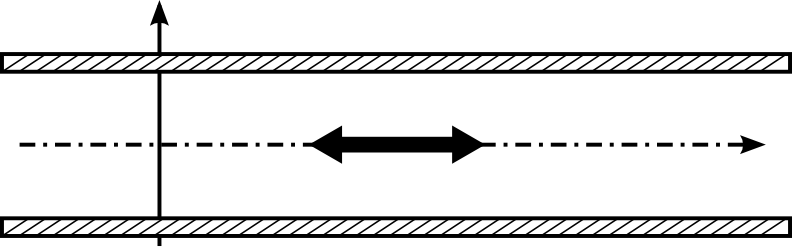
\includegraphics[width=10cm]{ecoulement_pulse_plan.png}}
  %    \put(14.5, 4.5){$-h$}
   %   \put(14.5, 18.5){$+h$}
   %   \put(35, 17){$\partial p/\partial x = K \cos \omega t$}
  %  \end{picture}
%  \end{center}
%  \mycaption{Ecoulement puls\'e en canal plan.}
%  \label{fig:ecoulement_pulse}
%\end{figure}


\comment{
\subsection{Bulles de savons connectées par une paille}


\begin{center}
\input{Figures/Bibulle.pspdftex}
\end{center}
Deux bulles de savon sont connectées par un tube cylindrique de rayon $a$
et de longueur $L$. On note $R_1(t)$ et $R_2(t)$ les rayons (intérieurs)
respectifs des bulles, $e$ l'épaisseur du film de savon, $P_1$ et $P_2$ 
les pressions à l'intérieur de chacune des bulles, et $P_0$ la pression 
atmosphérique.
Les viscosités cinématique et dynamique de l'air sont notés 
respectivement $\nu$ et $\mu$, et la tension interfaciale 
de l'interface film de savon / air est notée $\gamma$.

On suppose que $R_1$ et $R_2$ sont grands devant $a$ ; ainsi
le volume d'air contenu dans la bulle 1 sera pris comme égal
au volume d'une sphère de rayon $R_1$ (de même pour la bulle 2).

On note $V_0$ le volume total d'air dans les bulles 1 et 2.





\begin{enumerate}

\item
Exprimez $P_1-P_0$ en fonction du rayon $R_1$ et de l'épaisseur
$e$ du film de savon. Simplifiez cette expression en supposant $e\ll R_1$.
Exprimez de même $P_2-P_0$ en fonction de $R_2$.
%\begin{enumerate}

\item Quelles sont les solutions d'équilibre du système ? La situation $R_1 = R_2$ est-elle une situation stable ?


%En reprenant
%le calcul précédent et en comparant l'ordre de grandeur des termes
%visqueux et instationnaire dans l'équation de Navier-Stokes,
%montrez que l'approximation quasi-statique utilisée précédemment
%est effectivement valide si $\tau \gg a^2/\nu$.


\item On note $[T]$ l'échelle de temps du problème (inconnue à ce stade de la modélisation). 
Sous quelle(s) hypothèse(s) peut-on négliger le terme instationnaire et le terme d'advection dans l'équation de Navier-Stokes ?
%est effectivement valide si $\tau \gg a^2/\nu$.
%\end{enumerate}


\item
Montrez que sous les hypothèses formulées à la question précédente, l'écoulement dans
le tube est donné à tout instant par la loi de Poiseuille, et que le débit volumique
dans le tube (compté algébriquement dans la direction allant de la bulle
1 à la bulle 2) est donné par la formule suivante :

$$
Q = \frac{\pi a^4}{8 \mu L} (P_1-P_2)
$$



\item Montrez que le rayon $R_1(t)$ obéit à l'équation 
différentielle suivante :

$$
- \frac{d}{dt} \left( \frac{4 \pi R_1(t)^3}{3} \right) 
= \frac{\pi a^4\gamma }{2 \mu L} \left[ \frac{1}{R_1(t)} -     \frac{1}{R_2(t)}  \right]
$$

\item Sous quelle(s) hypothèse(s) est-il justifié de supposer que le volume
total d'air dans les bulles 1 et 2 est conservé ?
%Exprimez dans ce cas $R_2$ en fonction de $R_1$ et $V_0$ (volume total).

\item Le système admet une position d'équilibre correspondant à $R_1 = R_2 = R_0$ 
et $V_0 = 8 \pi/3 R_0^3$. On suppose que le système s'écarte légèrement 
de cette position d'équilibre et qu'on a $R_1(t) = R_0 + r(t)$ et $R_2(t) = R_0 - r(t)$.

Montrez que sous l'hypothèse $r(t) \ll R_0$ cette situation traduit bien la conservation du volume total. 


\item Par un développement limité de l'équation précédente, montrez que $r(t)$ 
obéit à une équation différentielle de la forme suivante :

$$
\frac{dr}{dt} 
= \sigma r , \qquad  \mbox{ avec } \sigma = \frac{a^4 \gamma}{4 R_0^4 \mu L} 
$$

\item Donnez la solution de cette équation. Quelle échelle de temps $[T]$ caractérisant l'évolution du système cette solution met-elle en évidence ?

%Exprimez $\sigma$ en fonction des données du problème.
%Que peut-on en déduire sur la stabilité de la position d'équilibre ?

\item
On donne les valeurs suivantes : $a = 1mm$, $R_0 = 5cm$, $\nu = 10^{-6} m^2. s^{-1}$, 
$\rho = 1.26 kg. m^{-3}$, $\gamma = 0.07 N.m^{-1}$, $L=20cm$. Calculez l'échelle de temps $[T]$ d'évolution du système. 
L'hypothèse quasi-statique est-elle bien justifiée ?
  }
 

\end{enumerate}



